% Finalizado 
\chapter{Conclusión}
\label{cap:conclusiones}

Como conclusión de este trabajo, se ha verificado tanto la viabilidad en el rendimiento del motor gráfico mediante la API Vulkan como la calidad visual de las simulaciones. 

Previamente al desarrollo del sistema de partículas, se realizaron diversas mejoras estructurales sobre el código base original (incluyendo la gestión de memoria mediante punteros inteligentes, el soporte para la carga de modelos tridimensionales, la interfaz de usuario y la optimización del proceso de compilación). 

Sentar esta infraestructura de base permitió centrar los esfuerzos directamente en la implementación del cálculo físico y renderizado de partículas en la GPU.

\section{Consecución de objetivos}

La meta del proyecto siempre fue la misma: conseguir que el programa fuera muy rápido incluso con mucha carga gráfica. La idea de pasarle todo el trabajo bruto a la tarjeta de vídeo parecía prometedora en la fase de diseño, y al final ha sido la clave. Ahora son esos pequeños trozos de código en la GPU los que se encargan de darle vida a cada punto, moverlo de sitio y borrarlo cuando toca.                      

Con esto se ha conseguido que el procesador se relaje bastante. Ya no tiene que estar mandando paquetes enormes de datos todo el rato. Al no tener ese atasco, el rendimiento es bastante bueno. No importal si pones fuego, humo o agua; la representación gráfica no sufre caídas de fotogramas en ningún momento.

\section{Resultados del sistema} 

Aparte de ir rápido tenía que verse bien (Ver Figura~\ref{fig:resultadoTodo}). Las matemáticas básicas que se usan dan unos resultados bastante buenos.
El humo crece como te esperas que lo haga, el fuego se mueve de una forma natural y el agua cae por su propio peso. 

Evidentemente, no hay un motor de físicas reales por debajo. Intentar hacer algo así hundiría el rendimiento. Únicamente se simulan partículas puntuales que obedecen un conjunto reducido de reglas básicas. Por eso hemos tenido que jugar con una ilusión optica. Queda visual, bonito y no satura el equipo.                                    


\begin{figure}[ht] 
    \centering
    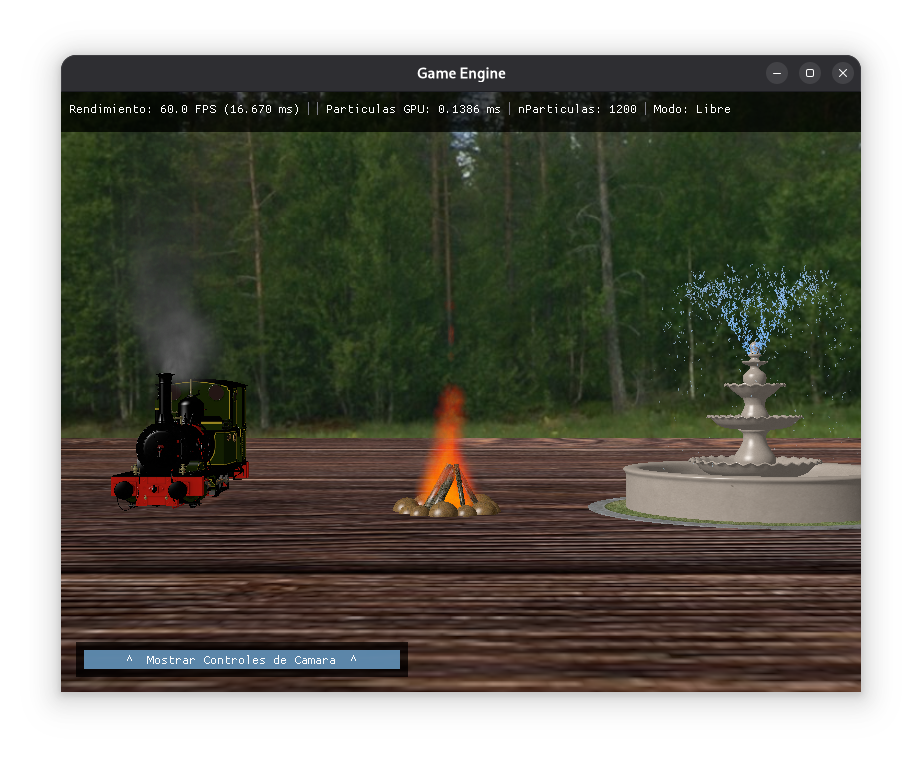
\includegraphics[width=0.85\textwidth]{Media/Conclusiones_4.png}
    \caption{Escena completa con los tres sistemas de partículas.}
    \label{fig:resultadoTodo} 
\end{figure}


\section{Trabajo futuro}

\noindent Como posibles trabajo futuro, se plantean las siguientes propuestas de mejora:

\begin{itemize}
    \item Incorporar algoritmos de ruido espacial para simular corrientes de viento. Esto aportaría mayor dinamismo al fuego, rompiendo su direccionalidad vertical y generando vórtices realistas.
    \item Implementar la detección de colisiones contra la geometría del escenario (como el suelo), lo que aumentaría la inmersión del entorno.
    \item Añadir cálculo de sombras dinámicas para mejorar la percepción de profundidad e iluminación global de la escena.
    \item Desarrollar un panel de control interactivo que permita ajustar los parámetros de simulación en tiempo real, evitando la necesidad de recompilar el código tras cada modificación.                                      
\end{itemize}



